\documentclass[times,12]{article}
\usepackage[margin=1in]{geometry}
\usepackage[hidelinks]{hyperref}
\usepackage{lineno}
\usepackage{amsmath}
\usepackage{hyperref}
\usepackage{graphicx}
\usepackage[round, comma]{natbib}
\usepackage{psfrag}
\usepackage[lofdepth,lotdepth]{subfig}
\usepackage{mathtools}
\usepackage{multirow, authblk}
\usepackage{bm}
\usepackage{physics}
\usepackage{xcolor}
\hypersetup{
    colorlinks,
    linkcolor={red!50!black},
    citecolor={blue!50!black},
    urlcolor={blue!80!black}
}

\bibliographystyle{apalike}


\title{Modeling the Dynamics of Pluto's Upper Atmosphere}
\author{Shane R. Carberry Mogan}
\affil{Mechanical and Aerospace Engineering Department\\
New York University Tandon School of Engineering\\
6 MetroTech Center, RH517D, Brooklyn, NY 11201}
\date{}

\begin{document}
\maketitle

\begin{abstract}
\noindent A spherically symmetric, globally averaged one-dimensional code is written to describe the dynamics of Pluto's upper atmosphere by solving fluid equations. The method applied, referred to as the Fluids-Jeans model, evolves physical properties of the gas according to various parameters, such as solar heating, up to a certain altitude in the rarefied regime of the atmosphere, the exobase. Upon obtaining values for these properties at the exobase, they are used to determine the concomitant Jeans molecular escape and energy outflow rates leaving Pluto's atmosphere. The Jeans escape rates are then used in the next iteration of solving the fluid equations to update values for the gas properties. This process is then iterated until convergence is achieved, at which point an accurate description of atmospheric escape can be established. The results of this code are compared to existing models in the literature and confirm that escape occurs on Pluto on a molecule-by-molecule basis.
\end{abstract}

\section*{Introduction}
\noindent The evolution of a planet's atmosphere is due in large part to the processes occurring in its upper atmosphere which drive escape. As a result of several ground-based telescopic and in-situ spacecraft observations, there is now a wealth of data available on the upper atmospheres of a number of topical solar system bodies, including Pluto. Prior to the NH flyby of the Pluto system in 2015, our understanding of its N$_2$ dominated atmosphere was largely based on rare occultation observations in 1988 (pre-perihelion), 2002, and 2006 (post-perihelion) \citep{Elliot2007, Young2008}. Thus, the data that would be obtained from the NH flyby was highly anticipated as part of its scientific objectives included characterizing the structure and composition of Pluto's atmosphere, quantifying its escape rate, and describing how it interacts with the surrounding space environment \citep{Stern2015, Gladstone2016, Bagenal2016}. Based on the encounter data, discoveries about Pluto's atmosphere relevant to this study included a colder upper atmosphere than expected; an extended atmosphere, albeit less than prior models predicted, with trace hydrocarbons; and updated escape rates, which inferred a drastically smaller rate for N$_2$ such that the dominant species lost was CH$_4$. Currently, the nominal models of Pluto's upper atmosphere published by the NH team \citep{Young2018} is typically only one-dimensional (1-D) and approximates the upper atmosphere by fitting the NH data. However, there still remains a clear lack of understanding of the evolution of Pluto's atmosphere. This discrepancy is predominantly attributed to the difficulty of readily simulating the physics driving escape from their upper atmospheres, even when using modern simulations software.\\
\indent Indeed, models of Pluto's atmosphere have been evolving for decades. It was was once widely believed to undergo escape in a process that was described as slow and hydrodynamic. Previous numerical models applied the concept of hydrodynamic escape by adapting the \textit{critical solution} of \cite{Parker1964} for planetary atmospheres to include heating by solar radiation \citep{Hunten1982, McNutt1989}. This adaptation, referred to as the slow hydrodynamic escape (SHE) model, was subsequently applied to Pluto \citep{Krasnopolsky1999, Strobel2008} and Titan \citep{strobel2008titan}. \cite{McNutt1989} used a self-consistent analytic approach to study the escape of CH$_4$ and CO from Pluto's atmosphere and found the escape rate was sensitive to solar extreme ultraviolet (EUV) heating. \cite{Yelle1997} accounted for the EUV heating as well as thermal conduction and viscous dissipation to numerically solve the fluid equations for the assumed hydrodynamic atmospheric escape of Pluto for N$_2$ and CO. \cite{Krasnopolsky1999} extended the analytic approach of \cite{McNutt1989} to include several more variables, such as the solar ultraviolet (UV) heating of Pluto's upper atmosphere. He then applied his approach to the assumed hydrodynamic escape of N$_2$ from Pluto with CH$_4$ diffusing upward through it and found substantial variations in the structure of the extended atmosphere as well as in the escape rates according to different solar cycles. \cite{Tian2005} solved the time-dependent hydrodynamic escape equations for a planetary atmosphere and applied them to the assumed hydrodynamic escape of N$_2$ from Pluto and derived a perihelion escape rate an order of magnitude higher than that of \cite{Krasnopolsky1999}. \cite{Strobel2008} solved the steady-state fluid equations for hydrodynamic escape and accounted for the EUV heat absorbed by N$_2$, the near-Infrared (IR) and UV heat absorbed by CH$_4$, and the rotational cooling by CO as a function of solar activity. \\
\indent The aforementioned calculations were all based on the assumption that the atmosphere was continuous, i.e., that intermolecular collisions dominated the overall flow, as in the lower, more dense regimes of the atmosphere. However, the continuum assumption fails when approaching a planet's exobase as collision frequencies diminish and the fluid equations fail to describe the flow of mass, momentum, and energy in an atmosphere \citep{Johnson2010, Volkov2011, Erwin2013}, which was shown to be critical for determining the structure of the upper atmospheres of Pluto and Titan \citep{Tucker2009, Tucker2012}. The region of validity for using the fluid equations is indicated by the Knudsen number (Kn = $l/H$), the ratio of the mean free path of molecules ($l = \frac{1}{\sqrt{2} n \sigma}$) to a characteristic length scale, which, for the purposes of modeling atmospheres, is set to an atmospheric density scale height ($H = \frac{r}{\lambda(r)}$). Here $n$ is the local number density, $\sigma = 1\times 10^{-14}$ cm$^{2}$ is the molecular cross section for N$_2$, $r$ is radial distance, and $\lambda(r)$ is the Jeans parameter, the ratio of the gravitational energy of a molecule ($\Phi_G = \frac{G M_P m}{r}$) to its thermal energy ($k_B T(r)$). The Jeans parameter is often used to characterize atmospheric escape rates, where $G = 6.67 \times 10^{-11} \frac{\mathrm{m^3}}{\mathrm{kg s^2}}$ is the gravitational constant, $M_P = 1.31 \times 10^{22}$ kg is the mass of Pluto,  $m = 28$ amu is the mass of a N$_2$ molecule, where an amu $=1.66 \times 10^{-27}$ kg, $k_B=1.38 \times 10^{-23} \frac{\mathrm{m^2 kg}}{\mathrm{s^2 K}}$ is the Boltzmann constant and $T(r)$ is radial temperature. The Knudsen number can be applied to divide an atmosphere into two kinetic regimes: (1) Kn $\geq$ 1, often referred to as the exosphere, where molecular collisions are rare but still critically important \citep{Marconi1996} and the molecules' ballistic trajectories can be traced using free molecular flow models \citep{Tucker2015}; and (2) Kn $<$ 1, henceforth referred to as the continuum regime, where collisions are sufficiently frequent over relevant length scales such that the gas in the atmosphere is kept in local thermodynamic equilibrium and fluid equations can accurately reflect its state \citep{Marconi1996, Erwin2013}. The idealized seperatrix between these regimes is often referred to as the exobase, which is typically taken to be at the altitude where Kn $\approx 1$ \citep{Tucker2012}. The transition between these regimes is difficult to determine and has been shown to require a molecular kinetic (MK) method to solve the Boltzmann equations \citep{Marconi1996} or by applying the direct simulation Monte Carlo (DSMC) method \citep{Bird1994}, as done by \cite{Tucker2009, Volkov2011, Volkov2011a, Tucker2012, Erwin2013, Tucker2015, Hoey2017a}. In theory, a MK method could be applied to all regimes of an atmosphere. However, due to the large number of intermolecular collisions at and below altitudes where Kn $<$ 0.1, such an approach would be computationally infeasible. Thus, dynamics of the continuum regime can instead be simulated by solving fluid equations which can then be iterated with MK methods above some pre-defined threshold \citep{Marconi1996, Tucker2012, Erwin2013}.\\
\indent Pluto's atmosphere has recently been demonstrated to undergo evaporative escape. That is, atmospheric escape occurs on a molecule-by-molecule basis \citep{Johnson2010, Volkov2011, Volkov2011a, Tucker2012, Erwin2013}. \cite{Tucker2012} modeled the continuum regime of the atmosphere with 1-D fluid equations before coupling them to a DSMC model of the upper atmosphere to constrain the thermally-driven escape. Therein the same temperature and density profiles were adopted as that of \cite{Strobel2008} and varying solar heating conditions were considered. They concluded that the thermally-driven escape from Pluto must be treated molecule-by-molecule. The standard analytic model for calculating evaporative escape was originally developed by \cite{Jeans1925} and is referred to as Jeans escape, where the corresponding escape rates depend primarily on the Jeans parameter. The Jeans molecular escape rate ($\left\langle \phi \right\rangle_J$) and energy escape rate ($\left\langle \phi_E \right\rangle_J$) are given as follows:
\begin{align}
\phi_J &= \pi r_x^2 n_x \left\langle v_{th,x} \right\rangle (1 + \lambda_x) \exp (-\lambda_x) \label{eq:Jeans1}\\
\left\langle \phi_E \right\rangle_J &= (k_B T_x) \left( 2 + \frac{1}{1 + \lambda_x} \right) \phi_J
\label{eq:Jeans2}
\end{align}
\noindent where $\left\langle v_{th,x} \right\rangle = \sqrt{\frac{8 k_B T_x}{\pi m}}$ is the mean molecular speed. Here the subscript $()_x$ refers to values at the exobase where these equations are typically applied as there are few collisions above this altitude to inhibit a molecule from escaping \citep{Erwin2013}. The Jeans molecular and energy escape rates obtained at the exobase can then be used to solve the fluid equations below this point to determine escape in an iterative process. Indeed, the Jeans escape boundary conditions (BCs) have been extensively used in modeling planetary atmospheres \citep{Chassefiere1996, Yelle2004, Tian2008, Erwin2013, Johnson2015}. This technique is applied herein to solve steady-state fluid equations in order to describe the atmospheric escape of Pluto.

\section*{Method}
\noindent The continuum regime of Pluto's is modeled via a set of fluid equations (conservation of mass, momentum and energy and an equation of state) for a single species (N$_2$), inviscid gas of constant molecular weight to give the radial dependence of number density ($n$), outward bulk velocity ($u$), and temperature ($T$). These equations assume a 1-D, spherically symmetric atmosphere where the gas properties are globally averaged and are functions of radial distance. The respective steady state equations for the conservation of mass, momentum and energy and equation of state are as follows:
\begin{align}
4 \pi r^2 n(r) u(r) &= \phi \label{eq:consmass}\\
n m \dv{}{r} \left( \frac{1}{2} u(r)^2 \right) + \dv{p(r)}{r} &= n(r) m \dv{\Phi_G(r)}{r}\\
\dv{}{r} \left( \phi \left(C_p T + \frac{1}{2}m u(r)^2 -\Phi_G(r) \right) - 4 \pi r^2 \kappa(T(r)) \dv{T(r)}{r} \right) &= 4 \pi r^2 q(r) \label{eq:consenergy}\\
p &= n k_B T
\end{align}
\noindent Here $\phi$ is the molecular escape rate through the 1D atmosphere to be measured at the upper boundary, $p$ is the pressure, $\kappa(T)$ is the thermal conductivity, $C_p = \frac{7}{2} k_B$ is the specific heat at constant pressure for a diatomic molecule, and $q(r)$ is the local heating/cooling rate per unit volume. For the conductivity term, the power law is applied to approximate the temperature dependence: $\kappa(T) = \kappa_0 T(r)^{\omega}$, where $\kappa_0 = 9.37 \times 10^{-5} \frac{\mathrm{W}}{\mathrm{m K^2}}$ and $\omega = 1$, to be consistent with \cite{McNutt1989, Strobel2008, Tucker2012, Erwin2013}. Recalling the equation of state, the conservation of momentum equation can be re-written as:
\begin{align}
\frac{dp}{p(r)} = - \left(\frac{G M_P m}{k_B T(r) r^2} + \frac{m \dv{u(r)^2}{r} }{2 k_B T(r)}\right) dr = - \left( \frac{\lambda(r)}{r} + \frac{m}{2 k_B T(r)} \dv{u(r)^2}{r} \right) dr
\label{eq:num}
\end{align}
\indent Solving Eqs. \ref{eq:consmass}, \ref{eq:consenergy}, and \ref{eq:num} requires four BCs. Consistent with \cite{Strobel2008, Tucker2012, Erwin2013}, the number density ($n(r_0) = n_0 = 4 \times 10^{-12}$ cm$^{-3}$) and temperature ($T(r_0)=T_0 = 88.2$ K) at the lower boundary ($r=r_0 = 1450$ km) are used. The additional two BCs required to describe an atmosphere with an open boundary have been discussed extensively. \cite{Tucker2012} described Pluto's N$_2$ atmosphere using a hybrid Fluid-DSMC model: first, the fluid equations derive values for $n(r)$ and $T(r)$ out to the exobase; upon reaching this altitude, the particle escape ($\phi$) and energy flow ($\phi_E$) are found using DSMC according to $n(r)$ and $T(r)$ at a selected radius in the upper atmosphere, $r(\mathrm{Kn} \approx0.1)$; the obtained values for $\phi$ and $\phi_E$ are then used to again solve the fluid equations out to the exobase; updated values for $n(r)$ and $T(r)$ at Kn $\approx 0.1$ are then inserted back into the DSMC model to obtain new values for $\phi$ and $\phi_E$. This iterative process is repeated until a converged solution for $n(r)$ and $T(r)$ is obtained. In a 1D atmosphere, upon finding the number density profile, $u(r)$ can be obtained from Eq. \ref{eq:consmass}. Alternatively, instead of including this additional method, the Jeans escape rates can be obtained at the exobase to be iteratively applied to the fluid equations. This approach is often referred to as the ``Fluid-Jeans'' method. \cite{Erwin2013} applied the Fluid-Jeans method to model atmospheric escape of Pluto to compare with the Fluid-DSMC model of \cite{Tucker2012}, and \cite{Johnson2015} applied this approach to calculate atmospheric escape for a number of Kuiper Belt Objects, including Pluto. Herein, the Fluid-Jeans method is applied to calculate escape from Pluto's atmosphere. The resultant fluid equations are given as follows:
\begin{align}
4 \pi r^2 n(r) u(r) &= \phi_J \label{mass}\\
n m \dv{}{r} \left( \frac{1}{2} u(r)^2 \right) + \dv{p(r)}{r} &= n(r) m \dv{\Phi_G(r)}{r} \label{momentum}\\
\dv{}{r} \left( \phi_J \left(\frac{7}{2} k_B T(r) + \frac{1}{2}m u(r)^2 -\Phi_G(r) \right) - 4 \pi r^2 \kappa(T(r)) \dv{T}{r} \right) &= 4 \pi r^2 q(r)\\
\end{align}
\noindent The equations for conservation of momentum and energy are then integrated with respect to radial distance to produce the following equations for $n(r)$ and $\dv{T(r)}{r}$:
\begin{align}
n(r) &= n_0 \left(\frac{T_0}{T(r)}\right) \exp \left[ - \int_{r_0}^r \left( \frac{\lambda(r)}{r} + \frac{m \dv{u(r)^2}{r} }{2 k_B T(r)}\right)dr \right] \label{eq:numdens}\\
\dv{T(r)}{r} &= \left( \frac{1}{4 \pi r^2 \kappa(T(r))} \right) \left[ - \left( \left\langle \phi_E \right\rangle_{r_0} + Q(r)\right) + \phi_J \left( \frac{7}{2} k_B T(r) + \frac{1}{2}m u(r)^2 - \Phi_G(r) \right) \right]
\end{align}
\noindent In a steady state atmosphere, conservation of energy requires that the energy carried off by escaping molecules ($\phi_E$) is replaced by a flow of energy into the lower boundary, $\left\langle \phi_E \right\rangle_{r_0}$, where $\left\langle \phi_E \right\rangle_{r_0} = \left\langle \phi_E \right\rangle_J  - Q_0$ \citep{Tucker2012}. Here $Q(r) = 4 \pi \int_{r_0}^r r^2 q(r) dr$ is the total heating rate above $r$ and $Q_0$ is the total heat deposited in the atmosphere from $r_0 \rightarrow r_{\mathrm{max}}$, such that $Q(r) \rightarrow Q_0$ as $r \rightarrow r_{\mathrm{max}}$. Most of the heat deposited by incoming photons goes into the lower regimes of the atmosphere and only a small fraction of this heat is carried away by escaping molecules, resulting in the atmosphere heating up. The local heating rate ($q(r)$) is given by:
\begin{align}
q_s(r) = \dv{F_s(r)}{r} = \chi_s \varepsilon_s \sigma_s n_s(r) F_s(r) \exp(-\tau_s(r) / \mu)
\end{align}
\noindent Here the subscript $()_s$ refers to the molecular species, where N$_2$ and CH$_4$ are considered; consistent with \cite{Strobel2008}, $\chi_{\mathrm{N}_2} = 0.97$ and $\chi_{\mathrm{CH}_4}=0.03$ are the fixed mixing ratios; consistent with \cite{Krasnopolsky1999}, $\sigma_{UV} = 1.8 \times 10^{-17}$ cm and $\sigma_{EUV} = 0.91 \times 10^{-17}$ cm are the absorption cross sections, which is attributed to solar heating absorbed by CH$_4$ and N$_2$ molecules, respectively, $\varepsilon_{\mathrm{N}_2} = 0.25$ and $\varepsilon_{\mathrm{CH}_4} = 0.5$ represent heating efficiency per photon absorbed, and $F_s(r)$ is the incoming energy flux at $\approx30$ astronomical units (AU) at a given altitude for solar UV and EUV minimum, mean, and maximum heating, which affect CH$_4$ and N$_2$ molecules, respectively; $\tau_s(r) = \int_{r_{\mathrm{max}}}^r \chi_s \sigma_s n_s(r) dr$ is the vertical optical depth; and $\mu = cos(60^{\circ}) = 0.5$ is used to approximate spherically averaged heating as the incoming solar heat fluxes reach Pluto at angles ranging from $0\rightarrow90^{\circ}$. Furthermore, consistent with \cite{Erwin2013}, to accommodate for the inefficient heating of a rarefied atmosphere, the heating rate is set to zero (i.e., the heating efficiency drops to zero) above $r_{\mathrm{max}}=r(Kn \approx 0.1)$. This initial model assumes a single-species, N$_2$ atmosphere ($n_s(r) = n_{\mathrm{N}_2}(r)$), but accounts for the influence of CH$_4$ via the concomitant UV solar heating. Thus, the final equation for determining the temperature profile is as follows:
\begin{align}
\dv{T(r)}{r} = \left( \frac{1}{4 \pi r^2 \kappa(T(r))} \right) \left[ - \bigg( \left\langle \phi_E \right\rangle_{J}  + \Delta Q_{\mathrm{N}_2} + \Delta Q_{\mathrm{CH}_4} \bigg) + \phi_J \left( \frac{7}{2} k_B T(r) + \frac{1}{2}m u(r)^2 - \Phi_G(r) \right) \right]
\label{eq:heating}
\end{align}
\noindent where $\Delta Q_s = Q_{s,0} - Q_s(r)$. For the case of no solar heating, (that is, when all of the incoming radiation is assumed to be absorbed below the lower boundary of this model) the Eq. \ref{eq:heating} simplifies to the following: 
\begin{align}
\dv{T(r)}{r} = \left( \frac{1}{4 \pi r^2 \kappa(T(r))} \right) \left[ - \left\langle \phi_E \right\rangle_{J} + \phi_J \left( \frac{7}{2} k_B T(r) + \frac{1}{2}m u(r)^2 - \Phi_G(r) \right) \right]
\label{eq:noheating}
\end{align}
\noindent The parameters used herein consistent with the literature are listed in Table \ref{tab:parameters}.
\begin{table}[h!]
\centering
\caption{Parameters used for various calculations according to corresponding molecular species.}
\begin{tabular}{lll}
\hline
Parameter & N$_2$ & CH$_4$ \\
\hline
\vspace{-0.1 in} \\
\vspace{0.05in} $\chi$ \citep{Strobel2008} & 0.97 & 0.03\\
\vspace{0.05in} $\sigma_{\mathrm{abs.}}$ [cm$^2$] \citep{Krasnopolsky1999} 	& $1.8 \times 10^{-17}$ & $0.91 \times 10^{-17}$	\\
\vspace{0.05in} $\varepsilon$ \citep{Krasnopolsky1999} & 0.25 & 0.50\\
\vspace{0.05in}$F_{\mathrm{Solar Min.}}$ [$\frac{\mathrm{ergs}}{\mathrm{cm}^2 \mathrm{s}}$] \citep{Krasnopolsky1999} & $1.7 \times 10^{-4}$ & $8.25 \times 10^{-4}$ \\
\vspace{0.05in}$F_{\mathrm{Solar Mean}}$ [$\frac{\mathrm{ergs}}{\mathrm{cm}^2 \mathrm{s}}$] \citep{Krasnopolsky1999} & $2.9 \times 10^{-4}$ & $1.4 \times 10^{-3}$\\
\vspace{0.05in}$F_{\mathrm{Solar Max.}}$ [$\frac{\mathrm{ergs}}{\mathrm{cm}^2 \mathrm{s}}$] \citep{Krasnopolsky1999} & $4.9 \times 10^{-4}$ & $2.4 \times 10^{-3}$\\
\vspace{0.05in}$r_0$ [km] \citep{Tucker2012} & 1450 & 1450\\
\vspace{0.05in}$n_0$ [cm$^{-3}$] \citep{Tucker2012} & $4 \times 10^{12}$ & $4 \times 10^{12}$\\
\vspace{0.05in}$T_0$ [K] \citep{Tucker2012} & 88.2 & 88.2\\
\hline
\end{tabular}
\label{tab:parameters}
\end{table}\\
\indent To initially solve the fluid equations for the no heating and solar minimum cases, the atmosphere is assumed to be isothermal ($T(r) = T_0$) and hydrostatic ($n = \frac{p}{k_B T_0}$) with no flow velocity ($u = 0$). Therefore, only the momentum equation is solved to determine $n(r)$:
\begin{align}
n(r) &= n_0 \exp \left[-\lambda_0 \left(1 - \frac{r_0}{r} \right)\right]
\label{eq:isothermnumdens}
\end{align}
\noindent Eq. \ref{eq:isothermnumdens} is continuously updated according to increasing $r$ until the exobase is achieved, at which point the Jeans escape rates are solved for according to Eqs. \ref{eq:Jeans1} and \ref{eq:Jeans2}. These obtained values are used in the next iteration to solve the full set of fluid equations for $n(r), u(r)$, and $T(r)$, where the atmosphere is no longer assumed to be isothermal and flow velocity is taken into consideration according to Eq. \ref{mass}. For the case of solar minimum heating, after locating the exobase, the corresponding number density profile is used to obtain $\tau(r)$ from $r(\mathrm{Kn} \approx 0.1) \rightarrow r_0$ using Simpson's method. Subsequently, the total heat deposited ($Q_0$) and the heating profile ($Q(r)$) are obtained from $r_0 \rightarrow r(\mathrm{Kn} \approx 0.1)$, also using Simpson's method. These terms are then used in Eq. \ref{eq:heating} to solve for $T(r)$ using a 4th order Runge-Kutta method. If no heating is considered, the steps for obtaining $\tau(r)$ and $Q(r)$ are ignored and Eq. \ref{eq:noheating} is solved for $T(r)$ using a 4th order Runge-Kutta method. Finally, $n(r)$ is obtained according to Eq. \ref{eq:numdens} using Simpson's method, after applying forward-difference, backward-difference, and central-difference formulae to solve $\dv{u(r)}{r}$ at $r_0$, $r$, and all radial points in between those bounds, respectively. These equations are then solved up to the exobase, at which point new values for the Jeans escape rates are obtained and used in the next iteration. This process is continued until convergence is achieved when a tolerance of $3\%$ is met between Jeans escape rates of current and previous iterations.\\
\indent For all heating cases, special treatment of the Jeans escape rates between iterations is required in order to prevent numerical instabilities and/or over-cooling over the atmosphere. Indeed, this is what led \cite{Erwin2013} to introduce time-dependence into their energy equation. However, the model used herein is able to obtain results for all but the solar maximum heating rate without introducing an unsteady equation for temperature. For the case of solar minimum heating, a relaxation parameter ($w$) is introduced when iterating Jeans escape rates. That is, when the Jeans escape rates are initially applied to the fluids equations ($F_{J,i} = \phi_{J,i}, \left\langle\phi_E\right\rangle_{J,i}$), they will produce new escape rates ($F_{J,k}$). The relaxation parameter is then applied to these two sets of rates before being entered into the next iteration: $F_{J,i+1} = (1-w) F_{J,i} + w F_{J,k}$, where $w=0.1$. Without this approach, as the atmosphere would heat up in one iteration, large Jeans escape rates would result. Subsequently in the next iteration, when applying those large Jeans escape rates, the atmosphere would over-cool, resulting either in numerical instabilities or a non-physical representation of the atmosphere. Therefore, $w$ prevents such instabilities from occurring and eventually results in convergence. When the heating rate increases from solar minimum to mean, however, additional treatment is required. For example, if one initially solves the fluid equations assuming an isothermal atmosphere, as was done for the no heating and solar minimum cases, to obtain Jeans escape rates to enter into the first iteration of the solar mean case, these rates are not large enough to cool the atmosphere to a point where an exobase can be numerically achieved. Hence, the converged Jeans escape rates obtained from the solar minimum case are applied as the initial rates for the solar mean case. However, even these rates are not large enough to reach Kn $\approx1$. Therefore, the heating rates are increased incrementally. As indicated in Table \ref{tab:parameters}, the value for solar mean is $\approx1.7 \times$solar minimum. Thus, the converged Jeans escape rates of the solar minimum case are first applied to $\approx 1.35 \times$solar minimum, roughly the average of solar minimum and mean, to obtain converged values at the exobase. Subsequently, the rates obtained by the $\approx 1.35 \times$solar minimum case are used to obtain converged rates for the solar mean case. This numerical issue only worsens when the heating rates further increase. Similar to the difference of solar mean to minimum, the solar maximum heating rate is $\approx 1.7 \times$solar mean. So a similar incremental increase of heating is applied, however, these increments have to be smaller in order to prevent numerical instabilities. The solar mean heating rate is subsequently increased by 1.1, 1.2, 1.25, 1.3, and 1.35, where converged rates from 1.1$\times$solar mean are entered into the 1.2$\times$solar mean case, and so on. This iterative process is repeated until 1.35$\times$solar mean, roughly the average of solar mean and maximum. When increasing heating beyond this rate, it seems no numerical treatment allows for converged Jeans escape rates or a numerical exobase to be achieved.\\
\indent The Fluid-Jeans model of \cite{Erwin2013} solved the unsteady fluid equations using an implicit time-stepping scheme for the cases of no heating and solar minimum, mean, and maximum heating. They compared these results against the SHE model of \cite{Strobel2008} and their other hybrid Fluid-DSMC model. Herein, the results of the steady Fluid-Jeans model is compared against these results for all but the solar maximum heating conditions, for reasons previously cited. However, trends from the results of no heating to 1.35$\times$solar mean heating cases are still used for comparison between models.
\section*{Results}
\noindent A 1-D Fluid-Jeans model is applied to the upper regimes of Pluto's atmosphere, starting from $r_0 = 1450$ km, where $n_0 = 4 \times 10^{12}$ cm$^{-3}$ and $T_0 = 88.2$ K, resulting in Kn$_0 \approx 10^{-6}$. This model iteratively evolves until reaching the exobase. Upon reaching this point, various parameters and profiles are obtained for comparison against existing models in the literature. For the purposes of this study, a globally averaged and spherically symmetric atmosphere is assumed. However, the upper atmosphere of Pluto is not spherical nor is its escape spherically symmetric. This is due to a number of factors, including non-uniform illumination, Charon's gravitational influence on Pluto's extended atmosphere, and centrifugal forces acting on the molecules in Pluto's atmosphere due to its rotation \citep{Tucker2015, Hoey2017}. Moreover, the magnitude of these effects change according to the varying solar insolation stemming from Pluto's highly elliptical orbit about the sun. Future work of this study will look to expand the current approach by using 2- and 3-D models such that it can include more of these factors.\\
\indent Results obtained for the no heating case agree relatively well with that of \cite{Erwin2013}, as shown in Table \ref{tab:noheat}. As spatial resolution is increased ($\Delta r = 1$ km $\rightarrow$ 0.5, 0.1 km), agreement between models is enhanced. Moreover, the higher the resolution, the less iterations were required for the model to reach convergence. However, the computational time required to run these higher resolution cases increased significantly. Regardless of resolution, smaller Jeans escape rates were obtained using the steady-state Fluid-Jeans (S-FJ) model compared to the unsteady Fluid-Jeans (U-FJ) model of \cite{Erwin2013}. The S-FJ model continued to predict less Jeans escape rates than the models of \cite{Erwin2013} as solar heating is introduced, again, regardless of resolution. Surprisingly, for the solar minimum case, as resolution increased to $\Delta r$ = 0.5 and 0.1 km, the overall heating of the atmosphere and ensuing escape rates diverged even further than what was predicted by \cite{Erwin2013}. That is, the atmosphere did not get as hot, which resulted in it being less extended and less molecules escaped. Furthermore, $\Delta r = 0.5$ and $\Delta r = 0.1$ km produced identical results. For that reason, coupled with the infeasible amount of computational time required to run such high resolution cases, only $\Delta r = 1$ km is considered for the remaining higher solar mean and $1.35 \times$ solar mean heating rates. Results of the solar minimum case with varying resolution compared to \cite{Erwin2013} are listed in Table \ref{tab:solarmin}.
Plots for no heating and solar minimum heating rates with varying resolution are shown in Fig. \ref{fig:varres}.\\
\newpage
\begin{table}[h!]
\centering
\caption{Comparison between results of the unsteady U-FJ model of \cite{Erwin2013} and the S-FJ model applied herein at varying spatial resolution of $\Delta r$ = 1, 0.5, and 0.1 km for no heating rates.}
\begin{tabular}{lllll}
\hline
& U-FJ & S-FJ ($\Delta r = 1$ km) & S-FJ ($\Delta r = 0.5$ km) & S-FJ ($\Delta r = 0.1$ km)\\
\hline \vspace{-0.1in}\\
$\phi$ [10$^{25}$ s$^{-1}$] & 35.0 & 26.4 (-24.6$\%$) & 29.4 (-16.0$\%$) & 31.6 (-9.71$\%$) \\
$r_x$ [km] & 3921 & 3896 (-0.64$\%$) & 3925 (+0.10$\%$) & 3946 (+0.64$\%$)\\
$\lambda_x$ & 8.71 & 8.89 (+2.1$\%$) & 8.77 (+0.69$\%$) & 8.69 (-0.23$\%$)\\
Iterations & - & 13 & 9 & 7\\
Computational time [s] & - & $\approx$75 & $\approx$210 & $\approx$4100 \\
\hline
\end{tabular}
\label{tab:noheat}
\end{table}
\begin{table}[h!]
\centering
\caption{Comparison between results of the unsteady U-FJ model of \cite{Erwin2013} and the S-FJ model applied herein at varying spatial resolution of $\Delta r$ = 1, 0.5, and 0.1 km for solar minimum heating rates.}
\begin{tabular}{lllll}
\hline
& U-FJ & S-FJ ($\Delta r = 1$ km) & S-FJ ($\Delta r = 0.5$ km) & S-FJ ($\Delta r = 0.1$ km)\\
\hline \vspace{-0.1in}\\
$\phi$ [10$^{27}$ s$^{-1}$] & 1.14 & 0.231 (-79.7$\%$) & 0.191 (-83.2$\%$) & 0.191 (-83.2$\%$) \\
$r_x$ [km] & 6900 & 5104 (-26.0$\%$) & 4858 (-29.6$\%$) & 4859 (-29.6$\%$)\\
$\lambda_x$ & 4.72 & 6.41 (+35.8$\%$) & 6.62 (+40.3$\%$) & 6.62 (+40.3$\%$)\\
Iterations & - & 14 & 10 & 8 \\
Computational time [s] & - & $\approx$280 & $\approx$14000 & $\approx$16000 \\
\hline
\end{tabular}
\label{tab:solarmin}
\end{table}
\begin{figure}[h!]
\centering
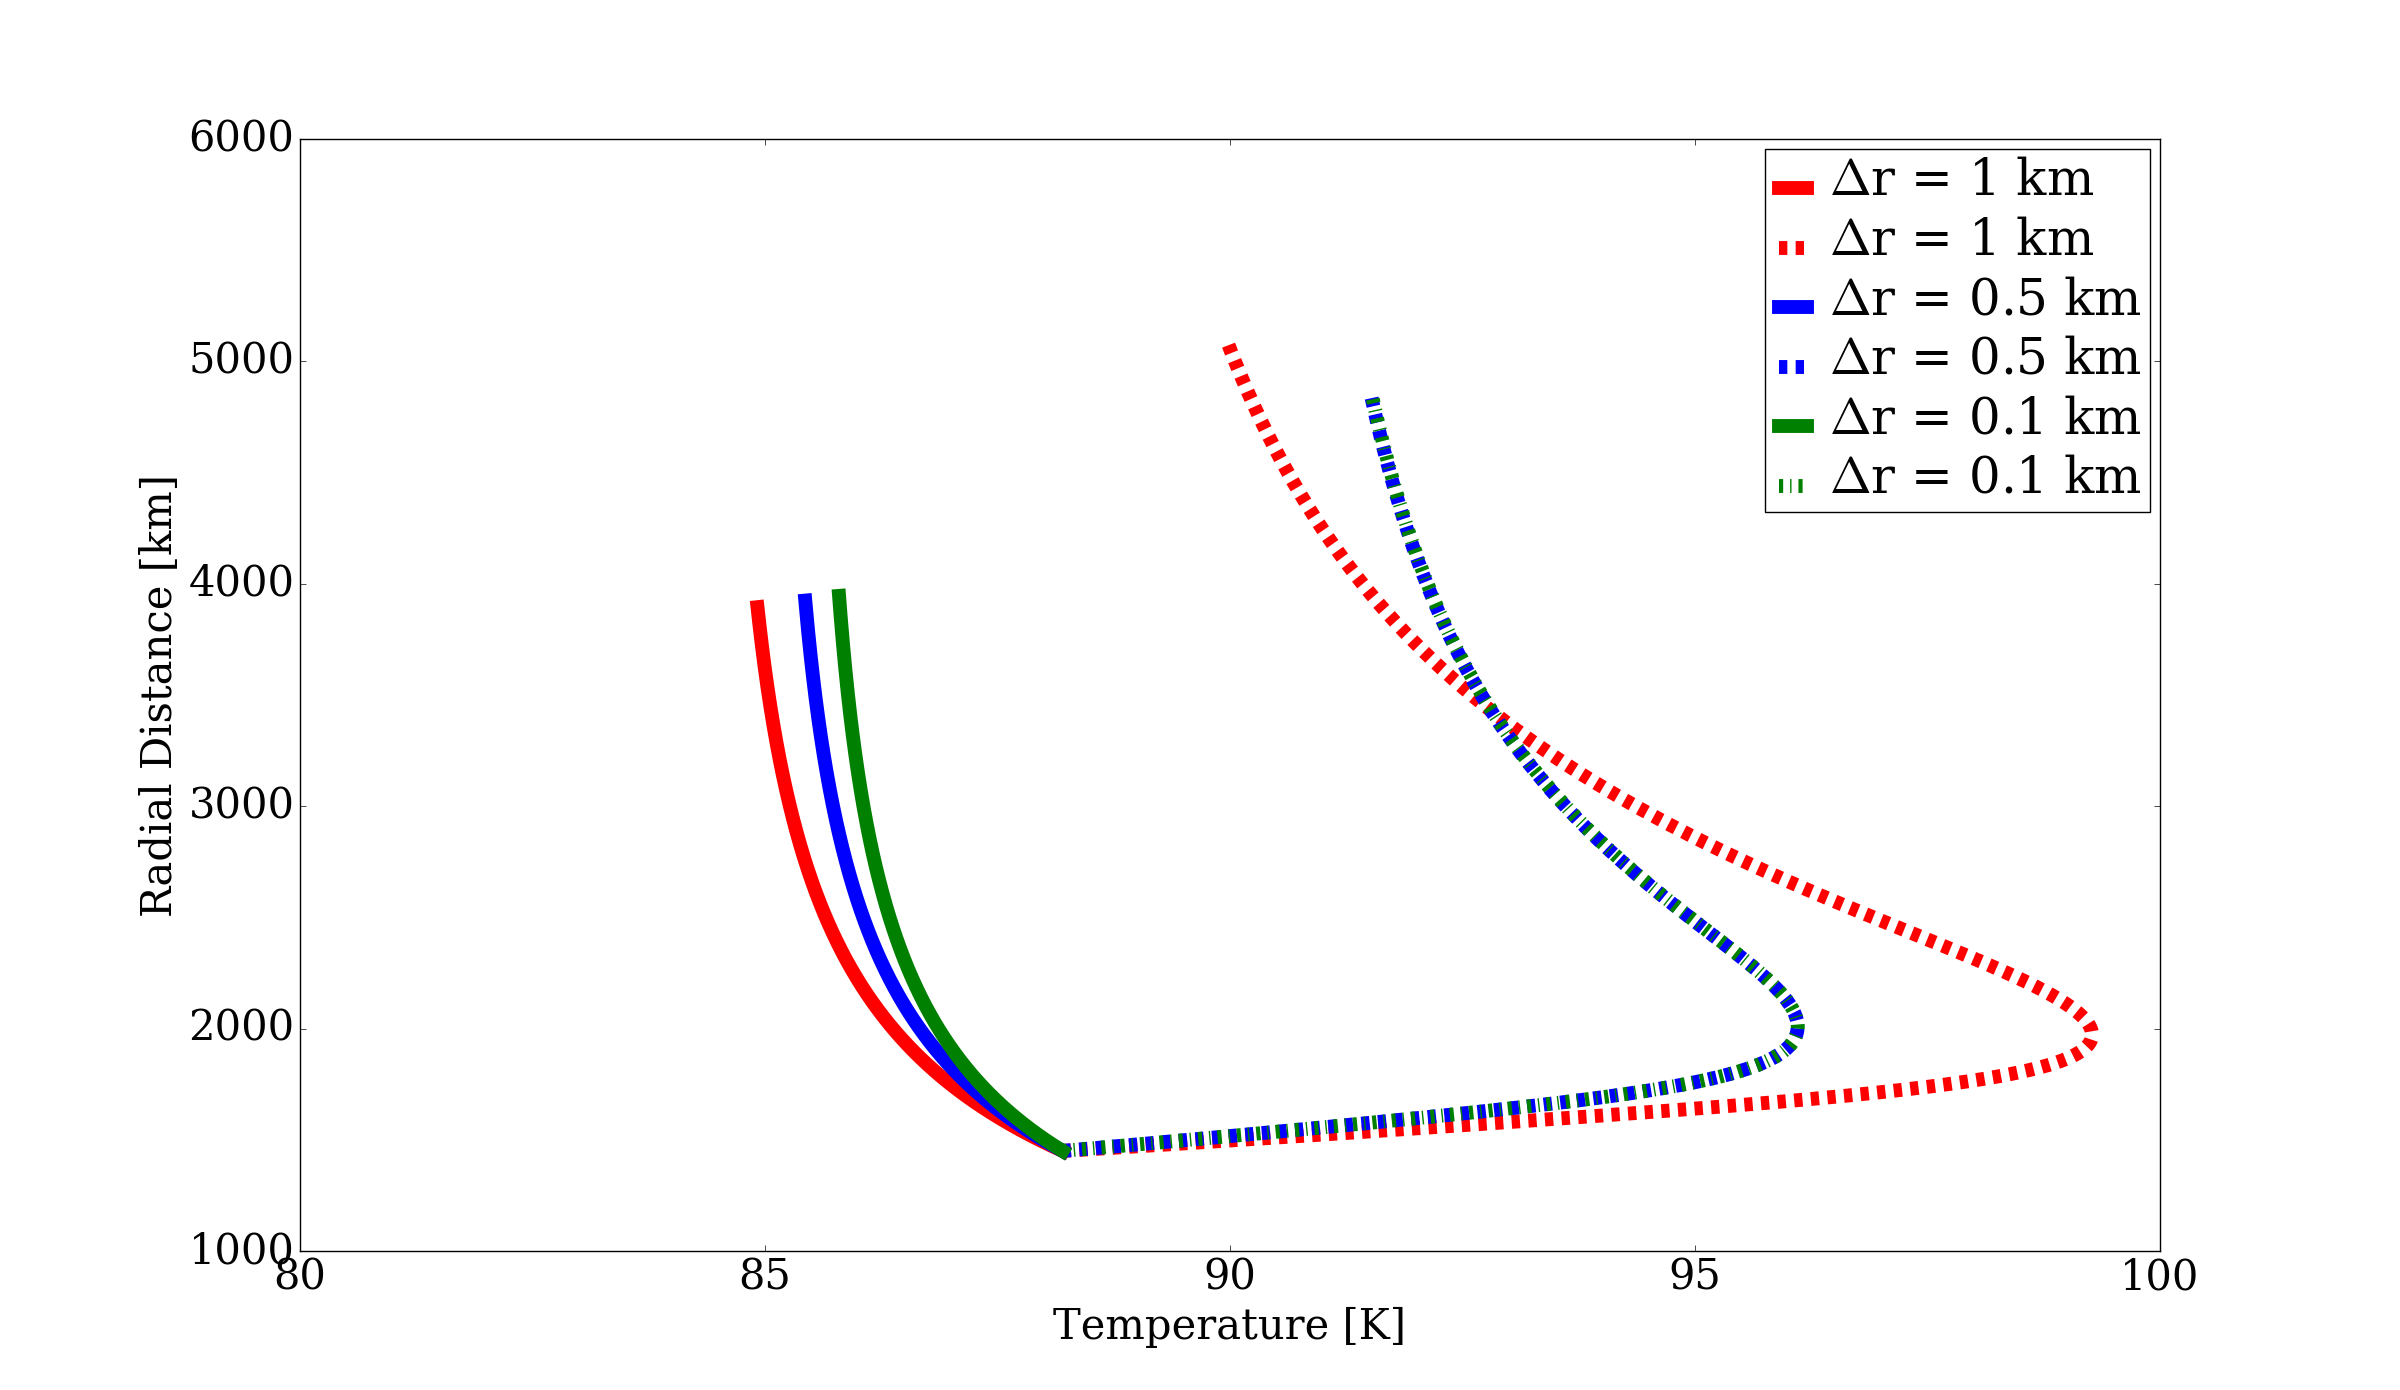
\includegraphics[scale=0.28]{../Figures/FluidJeans_NoHeatSolarMin_VarRes.png}
\caption{Comparison of no heating (solid lines) and solar minimum heating (dashed and dashed-dotted lines) rates for $\Delta r$ = 1, 0.5, and 0.1 km. The end of the lines indicate the altitude at which exobase is reached.}
\label{fig:varres}
\end{figure}
\indent As previously mentioned, the S-FJ model was unable to simulate the solar maximum heating case. However, as indicated by the trend between the solar mean and $1.35\times$solar mean in Fig. \ref{fig:nominmean135mean}, it appears as though the S-FJ would also under-predict results compared to the U-FJ model if results for the solar maximum case could be obtained. For reference and exact comparison, the results obtained by the S-FJ model are scaled to the same axes of the results of the U-FJ model, which are subsequently listed under the S-FJ plot in Fig. \ref{fig:nominmean135mean}. This allows for the rather dramatic difference between models to be visualized. Furthermore, Fig. \ref{fig:SFJUFJStrobelDSMC} shows the number density and temperature profiles of the S-FJ solar mean heating case scaled to the same axes of results obtained in \cite{Erwin2013} and \cite{Strobel2008}, which are listed below the S-FJ plot for comparison. The S-FJ model calculates a cooler atmosphere than the U-FJ, Fluid-DSMC, and SHE models. However, a higher exobase is obtained for the S-FJ model compared to the SHE model, albeit still less than that of the hybrid Fluid-DSMC and U-FJ models. Finally, a comparison between results obtained by the S-FJ and U-FJ are listed in Table \ref{tab:solarmeanmax}. As expected, based on the trends of the previous results, the S-FJ predicts a less extended atmosphere and concomitant smaller Jeans escape rates. \\
\indent Discrepancies between the S-FJ and U-FJ models are mostly attributed to the fact that the incoming heating fluxes were consistent with \cite{Krasnopolsky1999}, where globally averaged heating rates were applied. However, as in \cite{Strobel2008} and \cite{Erwin2013}, this was multiplied by a factor 2 to account for heating of Pluto specific to the side that was facing the Sun. That is, the heating rates used in the S-FJ model are half what was used in the U-FJ model. If, however, the heating rates were to be doubled in the S-FJ model, then numerical instabilities would arise in earlier iterations and would potentially not be able to simulate solar mean or even minimum heating rates. For example, solar mean heating rates were able to be simulated in the S-FJ model, which is $\approx 1.7 \times$ solar minimum heating rates. If the solar minimum heating rates were then multiplied by 2, as in \cite{Strobel2008} and \cite{Erwin2013}, maintaining stability is not guaranteed even for this initial case, as this proved to be an issue when increasing heating rates from solar mean in the S-FJ model. However, given that NH actually observed cooler temperatures in Pluto's upper atmosphere than was previously predicted, this globally averaged heating rate might actually be more realistic.\\
\indent Furthermore, other discrepancies could be attributed to the special treatment (e.g., incremental heating and introducing a relaxation parameter) required to prevent numerical instabilities. Indeed, this tedious, additional work is what led \cite{Erwin2013} to solve the fluid equations by re-introducing time-dependence. Furthermore, a different value for tolerance was used in \cite{Erwin2013} than in this model. Therein, convergence was obtained when the change in temperature multiplied by the time step size divided by the number of radial grid points was less than $10^{-5}$ K/s. However, \cite{Tucker2012}, who similarly calculated the continuum regime of Pluto's atmosphere solving fluid equations before iterating with DSMC, obtained convergence when temperature and density agreed within 3$\%$ in the region where these two methods overlapped. This latter approach is what led to a 3$\%$ tolerance being applied herein, albeit to Jeans escape rates. If a $10^{-5}$ tolerance were applied, then perhaps the results listed are not in fact converged values and would be subject to change, hopefully to more closely reflect the results of the U-FJ model. However, this would require several more iterations to achieve such a tolerance, thus falling outside of the time-frame required for this model. This could also cause the relaxation parameter to be dynamically altered, resulting in potentially many more trial-and-error cases. Surprisingly, when a higher resolution was implemented for the S-FJ model, the results actually further diverged from the U-FJ model, which showed no difference between $\Delta r=0.1$ km and $\Delta r = 0.5$ km. \cite{Tucker2012} and \cite{Erwin2013} implemented a varying step size when solving for the fluid equations to better simulate the heating in the lower altitudes of their models. However, this proved to be unnecessary as higher resolution resulted in less accurate results, and, hence, a constant $\Delta r=1$ km was used throughout the S-FJ model. Another cause for discrepancy could be attributed to the various constant values used. Nowhere in \cite{Tucker2012} or \cite{Erwin2013} do they specify their collisional cross-section for a N$_2$ molecule ($\sigma$), nor do they specify what exactly they used for the mass of Pluto ($M_P$). The collisional cross-section used in this study was the same one used by \cite{Johnson2015} and the mass of Pluto used was found on a NASA website (nssdc.gsfc.nasa.gov/planetary/factsheet/plutofact.html). These differences could result in large changes over the many calculations performed per case. Moreover, other heating and cooling mechanisms provided by CH$_4$ absorption of near-infrared (IR) and CO rotational line emissions, respectively, were neglected despite being considered in the U-FJ model. However, \cite{Erwin2013} showed these additional mechanisms to be negligible in comparison to the UV and EUV absorption. Regardless of these discrepancies, the results obtained by the S-FJ model confirm the results of \cite{Tucker2012} and \cite{Erwin2013}. That is, atmospheric escape on Pluto does is not hydrodynamic and occurs on a molecule-by-molecule basis.\\
\begin{table}[h!]
\centering
\caption{Comparison between results of the unsteady U-FJ model of \cite{Erwin2013} and the S-FJ model applied herein for solar mean, $1.35 \times$solar mean and solar maximum heating rates.}
\begin{tabular}{lllll}
\hline
& U-FJ (Solar Mean) & U-FJ (Solar Max) & S-FJ (Solar Mean) & S-FJ ($1.35\times$Solar Mean)\\
\hline \vspace{-0.1in}\\
$\phi$ [10$^{27}$ s$^{-1}$] & 2.58 & 5.81 & 0.452 (-82.4$\%$) & 0.692 \\
$r_x$ [km] & 9315 & 14260 & 5878 (-$36.9\%$) & 6588\\
$\lambda_x$ & 3.84 & 3.01 & 5.63 (+46.6$\%$) & 5.14 \\
\hline
\end{tabular}
\label{tab:solarmeanmax}
\end{table}
\begin{figure}[h!]
\centering
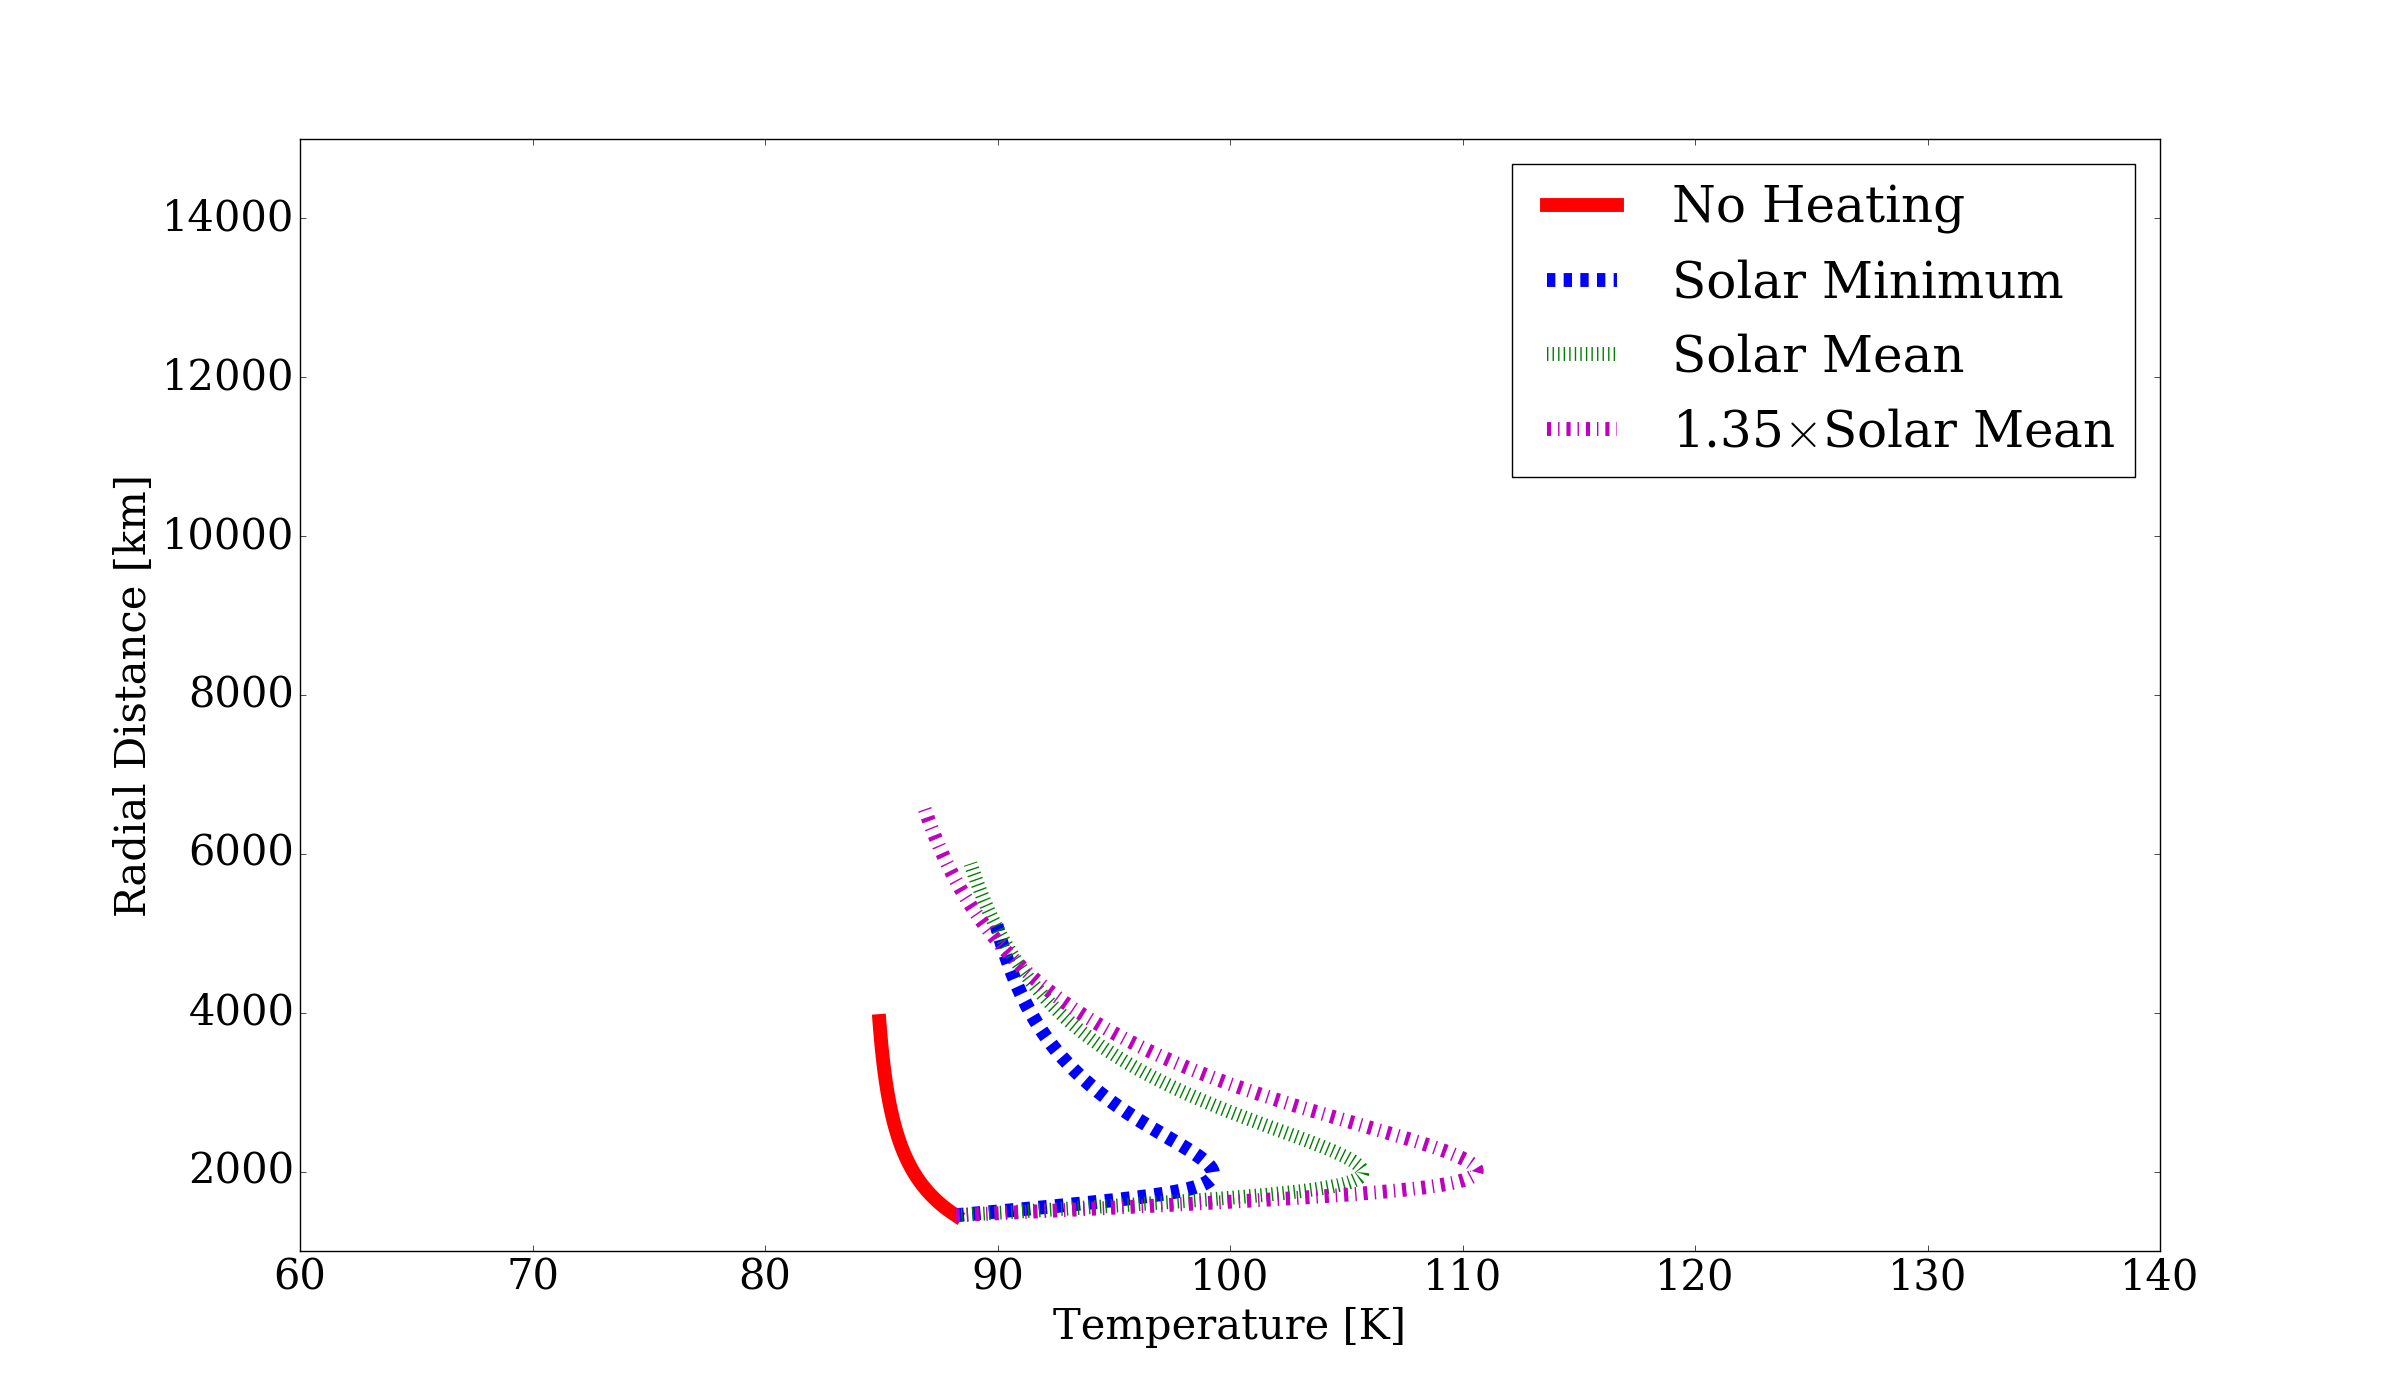
\includegraphics[scale=0.22]{../Figures/FluidJeans_NoHeatSolarMinMean135Mean.png}\\
\includegraphics[scale=1.38]{../Figures/Erwin_2_2013.jpg}
\caption{ (\textit{Top:}) Results obtained by the S-FJ model for no heating, solar minimum, mean, and 1.35$\times$solar mean heating rates. (\textit{Bottom}:) Results obtained by \cite{Erwin2013} for no heating, solar minimum, mean, and maximum heating rates. The end of the lines indicate the altitude at which exobase is reached.}
\label{fig:nominmean135mean}
\end{figure}
\begin{figure}[h!]
\centering
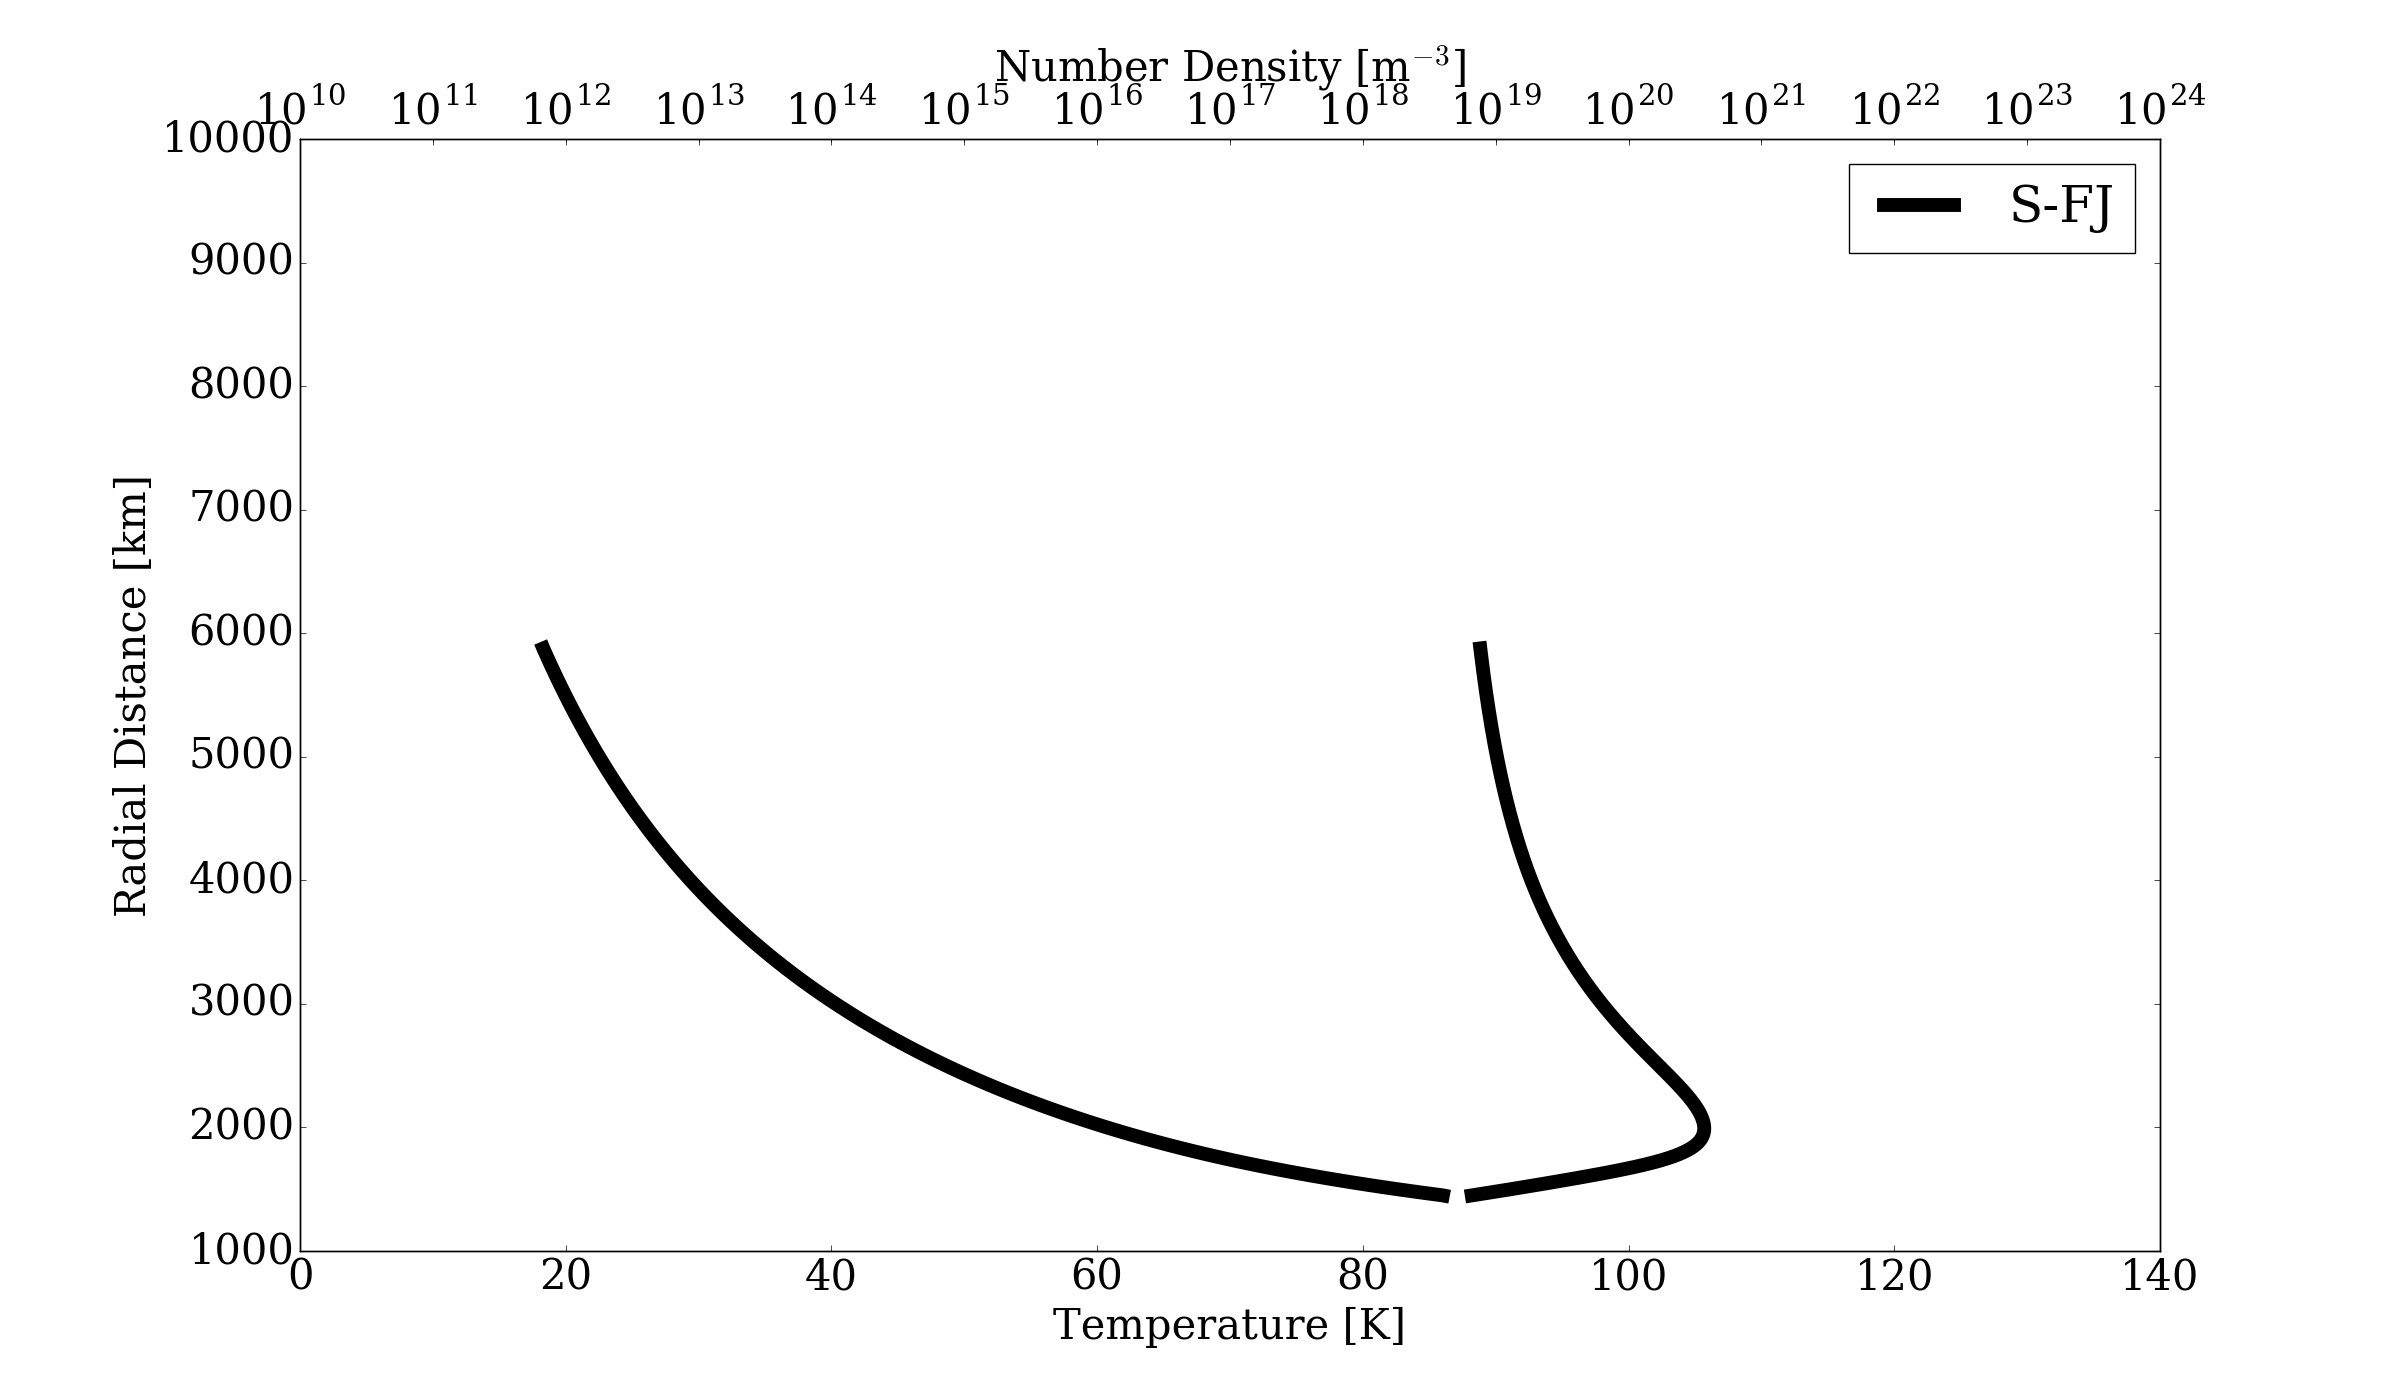
\includegraphics[scale=0.25]{../Figures/NumDens_Temp_Rad_SFJ.png}\\
\includegraphics[scale=1.45]{../Figures/Erwin2013.jpg}
\caption{ (\textit{Top:}) Number density and temperature profile obtained by the S-FJ model for the solar mean heating rate. (\textit{Bottom}:)  Number density and temperature profiles obtained by the U-FJ and hybrid Fluid-DSMC models of \cite{Erwin2013} and the SHE model of \cite{Strobel2008} for the solar mean heating rate. The end of the lines indicate the altitude at which exobase is reached. Here, $r_t$ represents the point at which the transition between the fluid equations and DSMC takes place, and $r_s$ represents the altitude at which the sonic point is reached.}
\label{fig:SFJUFJStrobelDSMC}
\end{figure}
\pagebreak

\newpage
\section*{Conclusion}
\noindent A steady-state Fluid-Jeans model was solved for modeling the upper atmosphere of Pluto in order to characterize atmospheric escape. The Fluid-Jeans model uses the Jeans escape rates as upper boundary conditions for solving steady-state fluid equations. Once obtained, the Jeans escape rates are applied to these equations in subsequent iterations until converged values are achieved. When compared to the same results produced by a Fluid-Jeans model that solved unsteady fluid equations, results varied depending on the heating rates. For the case of no heating, as resolution increased, the Jeans parameter and escape rates better agreed with the unsteady Fluid-Jeans model. However, when solar heating was introduced, as resolution increased, the results further diverged from the unsteady model. That is, the atmosphere got even cooler. The results calculated by the steady model assumed heating rates about half that of the unsteady model and thus predicted a less extended atmosphere with concomitant cooler temperatures and lower escape rates. Despite this difference in heating rates, a similar trend in the temperature profile was demonstrated. In addition, a more extended atmosphere was still predicted than by slow hydrodynamic escape models. Thus, Pluto's escape is confirmed not to be hydrodynamic but occur on a molecule-by-molecule basis.

\section*{Future Work}
\noindent The steady-state Fluid-Jeans model used herein and the aforementioned models within the literature are all 1-D, under the assumption that the atmosphere and its escape spherically symmetric, and globally average the physical properties. More advanced, hybrid models in the literature are confined to similar simplifications. Even the state of the art model for Pluto's upper atmosphere, which has been fitted to the observations of the NH flyby, is typically only 1-D. However, due to a number of factors involving Pluto's planetary dynamics as well as its surrounding space environment, neither its atmosphere nor its escape are spherically symmetric. Therefore, the way Pluto's upper atmosphere is modeled needs to be dramatically changed. Indeed, the remainder of my PhD will be focused on creating more realistic models of Pluto's upper atmosphere to better account for these factors by expanding to 2- and 3-D. 

Modeling an atmosphere in 2-D can account for which side of Pluto is facing the sun (i.e., its ``day-side''). Previously, this was taken into account by applying a global average \citep{Strobel2008, Erwin2013}. However, the day-side of Pluto's atmosphere, bearing the brunt of the incoming solar radiation, would be more extended than on the side not facing the sun (i.e., its ``night-side''), resulting in an asymmetric shape. This issue only worsens when expanding to a 3-D model as Pluto's rotation about its axis is factored in, resulting in more complex flow. In addition, expanding a Pluto atmospheric model to multiple dimension can become even more complicated as Charon's gravitational influence can also play a role in its asymmetric expansion and escape as the two planetary bodies revolve about their barycenter \citep{Tucker2015, Hoey2017a}. \cite{Hoey2017a} generated 3-D models of Pluto's rarefied regimes solely using the DSMC method to account for these variables, but at great computational cost. Therein, however, they stressed the importance for improved models of the continuum regime and better synergy at the continuum-rarefied boundary for hybridization purposes. Indeed, properly modeling this transition from collision-dominated to rarefied regimes of an atmosphere has been shown to be critical for determining the structure of Pluto's upper atmosphere and its escape rates \citep{Tucker2009, Tucker2012}.\\
\indent If a hybrid model were expanded to 2- or 3-D, then a single transition altitude would not suffice, as it does in 1-D models. That is, the shape of the atmosphere and, hence, the region where transition between methods is required would vary. This makes coupling methods complicated when dealing with grid-based methods, such as the finite-difference schemes previously used to solve the fluids equations \citep{Strobel2008, Tucker2012, Erwin2013} or the DSMC \citep{Bird1994}. For example, the grid used to solve the fluid equations would be more extended in some regions of the atmosphere and less so in others, resulting in the DSMC grid delving deeper into the atmosphere in some regions than in others. Moreover, these complicated shapes would vary over time due to dynamic physical parameters. Indeed, maintaining connectivity of grids over regions with moving interfaces or complicated geometries has been shown to be difficult without introducing numerical errors \citep{liu2010, ni2016}. These computational issues have resulted in the proliferation of particle-based methods, which do not require a grid but instead represent the domain by dividing it into discrete fluid elements, referred to as particles \citep{monaghan1992, monaghan2005}.\\
\indent In particle-based methods, each particle represents its own system of equations which evolve according to its surrounding environment of similarly represented particles according to the governing dynamics. The local density of a particle of interest (PoI) is calculated based on a sampling rate of the mass distribution. However, this can lead to noise as the density estimate will be sensitive to whether a distant particle is in- or outside of the estimate. This issue is specifically dealt with by the Smoothed Particle Hydrodynamics (SPH) method, where neighboring particles' contributions to the PoI are weighted according to their relative distances. That is, the closer the particles are to each other, the larger their influence on the local density estimate; and the farther the particles are from each other, the smaller their influence. Thus, the density estimate is \textit{smoothed} \citep{Price2012}. Neighboring particles' influence on a PoI is expressed as a function (i.e., the ``smoothing function'') of the non-dimensional relative distances between particles. The smoothing function is given by the ratio of the distance between two given particles and the ``smoothing length.'' The smoothing length controls the size of the influence domain surrounding the PoI in which neighboring particles are to be considered \citep{liu2003}. SPH was originally invented to simulate non-axisymmetric phenomena in astrophysics \citep{gingold1977, lucy1977}. In recent years, it has gained significant popularity in the field of computational fluid dynamics, due to its purely Lagrangian nature and its capability in dealing with free-surfaces and interfaces, as well as large deformations \citep{monaghan1994, monaghan2005, ni2016}. In addition, SPH has recently demonstrated compatibility with the parallel computing power of graphics processing units (GPUs) in order to simulate large-scale phenomena that would otherwise require high computational resources \citep{dominguez2013, crespo2015}. \\
\indent Thus, SPH is the ideal method to simulate Pluto's collision-dominated atmosphere up to the dynamic interface between continuum and rarefied regimes, before transitioning to a MK method in the latter regime. Indeed, coupling these two methods in a dynamic manner in order to simulate Pluto's asymmetric upper atmosphere will be the focus of my PhD research.

\section*{Acknowledgments}
\noindent I would like to personally thank Dr. Robert Johnson, for his guidance and patience in assisting me on this project. Without his knowledge and experience on this topic, among many, many other topics, and his ingenuity towards obtaining physical results, I would surely be lost in this endeavor of attempting to re-produce some of his earlier work. I would also like to thank Christopher Tiede for his patience and expertise in being able to assist me in making my code more efficient, as well as for helping me on several earlier assignments. Finally, I would like to thank Prof. Andrew MacFadyen for allowing me to take Computational Physics in the first place. This class has taught me an innumerable amount when it comes to being able to simulate physical phenomena, no matter how daunting they may initially seem. Thus, I highly recommend this class, especially when taught by this professor, to anyone who is interested in an education or career in computational mathematics, science, physics, or engineering.

\newpage
\bibliography{CompPhys}
\end{document}